%!TEX root = ../dokumentation.tex
\chapter{Machbarkeitsstudie}\label{chap:machbarkeitsstudie}
Ziel der Machbarkeitsstudie ist es, Informationen über die Schwierigkeit des Entwurfs und der Herstellung eines \ac{LIDAR} Sensors mittels einer Photodiode zu erlangen. 

\section{Versuch 1: Test handelsüblicher Photodioden}
In einem ersten sehr einfachen Aufbau wurde der Photostrom in einer Handelsüblichen Photodiode gemessen.
\subsection{Versuchsaufbau}
\subsubsection{Verwendete Bauteile}

\begin{table}[H]
	\centering
	\caption{Bauteilliste Versuch 1}
	\begin{tabular}{|l|l|}
		\hline
		\textbf{Bezeichnung} & \textbf{Bauteil (Beschreibung)}
		\\\hline
		Photodiode & PD333-3C/HO/L2 EVL
		\\\hline
		Laserpointer & 1mW, 630-680 nm
		\\\hline
		Taschenlampe & 
		\\\hline
	\end{tabular}
\end{table}

\subsubsection{Verwendete Messgeräte}
\begin{table}[H]
	\centering
	\caption{Messgeräteliste Versuch 1}
	\begin{tabular}{|l|l|}
		\hline
		\textbf{Art des Messgeräts} & \textbf{Bezeichnung}
		\\\hline
		Digitalmultimeter & Agilent
		\\\hline
		DC Spannungsquelle &
		\\\hline
	\end{tabular}
\end{table}
\subsubsection{Aufbau}
Wie in Kapitel \ref{sec:photodioden} beschrieben müssen Photodioden mit einer Sperrspannung betrieben werden, um einen möglichst großen Photostrom messen zu können, daher wurde die Photodiode mit einer Sperrspannung von $5V$ betrieben. Das Digitalmultimeter wurde in Reihe zur Photodiode geschlossen um den entstehenden Photostrom messen zu können.\\
Um direkt einen möglichst guten Eindruck der späteren Anwendung zu bekommen wurde direkt ein Testaufbau verwendet, in welchem das Licht vom Laserpointer reflektiert und danach von der Photodiode detektiert wird. Dazu wurde die Photodiode direkt neben dem Laserpointer positioniert (Abbildung: \ref{versuch1_versuchsaufbau}). 
\begin{figure}[H]
	\centering
	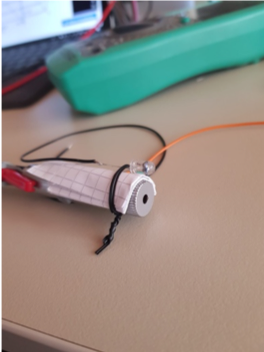
\includegraphics[width=0.25\textwidth]{images/Machbarkeitsstudie/Versuch1_Aufbau}	
	\caption{Versuchsaufbau}
	\label{versuch1_versuchsaufbau}
\end{figure}
\subsubsection{Messungen}
Insgesamt wurden vier Messungen durchgeführt.
\begin{enumerate}
	\item Photostrom im nicht abgedunkelten Raum
	\item Photostrom im abgedunkelten Raum
	\item Photostrom bei direktem Beleuchten mit einer Taschenlampe
	\item Photostrom bei direktem Beleuchten mit einem Laserpointer
	\item Photostrom bei Reflexion von einem Laserpointer
\end{enumerate}
Diese ersten vier Messungen sollen einen ersten Überblick über die Stärke des Photostroms geben und die Störeinflüsse des Umgebungslicht näher betrachten. Zudem kann über die fünfte Messung und die Variation des Abstandes der Reflexionsfläche Information darüber erlangt werden, wie groß die relative Änderungen des Photostroms bei relativer Änderung des Abstandes ist.
\subsection{Beobachtung}
Die größte Beobachtung, welche bei den Messungen gesehen werden konnte ist, dass der Photostrom nur im Bereich von wenigen $\mu A$ liegt.
\begin{enumerate}
	\item Nicht abgedunkelter Raum: $15\mu A$ 
	\item Abgedunkelter Raum: $3-5\mu A$  (sogenannter Dunkelstrom)
	\item Lichteinstrahlung Taschenlampe: $80\mu A$ 
	\item Lichteinstrahlung Laserpointer: $200\mu A$
\end{enumerate}
Diese ersten vier Messungen zeigten bereits, dass die Auftretenden Photoströme nur sehr gering sind und daher zusätzlich zu einer sehr schnellen Auswerteelektronik (Messung nach dem \ac{ToF} Prinzip) zudem eine sehr genaue Verstärkerschaltung nötig ist um gute Messergebnisse zu erzielen.
\begin{enumerate}
	\setcounter{enumi}{4}
	\item Bei Änderung des Abstandes der Reflexionsfläche in Messung fünf kann festgestellt werden, dass ein Abstand bis ca. $7cm$ detektiert werden kann. Die relative Änderung des Photostroms beträgt dabei $\frac{0,2}{7}\frac{\mu A}{cm}$
\end{enumerate}
\subsection{Erkenntnis}
Die größte Erkenntnis aus den Messungen des ersten Versuchs ist, dass Störende Lichteinflüsse so gut wie möglich eliminiert werden müssen. Dies kann z.B. durch Filter, welche nur das vom Laser ausgesandte Licht durchlassen, realisiert werden.\\
Ein Weiterer Punkt welcher festgestellt wurde ist, wie bereits schon erwähnt wurde, dass eine sehr Präzise Schaltung zu Feststellung der Photoströme nötig ist, da die Änderungen in sehr geringen Bereichen geschehen. Eine Lösung für dieses Problem könnte eine Verstärkerschaltung aus hochpräzisen Operationsverstärkern sein.\\
Der Dritte Punkt welcher in folgenden Messungen betrachtet werden sollte ist, dass eine Diode mit einer höheren Empfindlichkeit gegenüber der Lichteinstrahlung hat. Da wie beobachtet wurde die Reflektierte Lichtmenge sehr gering ist. Hier könnte beispielsweiße eine Avalanche Photodiode verwendet werden.

\section{Versuch 2: Weiterer Test handelsüblicher Photodioden}
\subsection{Versuchsaufbau}
\subsubsection{Verwendete Bauteile}
\begin{table}[H]
	\centering
	\caption{Bauteilliste Versuch 2}
	\begin{tabular}{|l|l|}
		\hline
		\textbf{Bezeichnung} & \textbf{Bauteil (Beschreibung)}
		\\\hline
		Photodiode & BPW34
		\\\hline
		Laserpointer & 1mW, 630-680 nm
		\\\hline
		Karton & 
		\\\hline
		Lupe &
		\\\hline
	\end{tabular}
\end{table}

\subsubsection{Verwendete Messgeräte}
\begin{table}[H]
	\centering
	\caption{Messgeräteliste Versuch 2}
	\begin{tabular}{|l|l|}
		\hline
		\textbf{Art des Messgeräts} & \textbf{Bezeichnung}
		\\\hline
		Digitalmultimeter & Agilent
		\\\hline
		DC Spannungsquelle & 
		\\\hline
	\end{tabular}
\end{table}
\subsubsection{Aufbau}
In die Seite des Kartons wurde je ein Loch für Laserpointer und Photodiode geschnitten und diese jeweils darin Angebracht. Im Karton wurde eine Reflexionsfläche im Abstand von $7cm$ aufgestellt und der Karton wurde verschlossen. Die Diode wurde mit einer Sperrspannung von $5V$ betrieben und das Digitalmultimeter in Reihe zur Photodiode geschaltet um analog zu Versuch 1 den entstehenden Photostrom zu messen. 
\subsubsection{Messungen}
\begin{enumerate}
	\item In der ersten Messung wurde die Photodiode zusammen mit dem Laserpointer im Dunklen getestet und der Photostrom im Dunkeln sowie bei Betätigung des Laserpointers gemessen.
	\item In einer zweiten Messung wurde vor der Photodiode eine Lupe Positioniert, sodass das Licht auf die Photodiode gebündelt wird. Es wird erwartet, dass durch die Lupe ein größerer Photostrom entsteht.
\end{enumerate}
\subsection{Beobachtung}
\begin{enumerate}
	\item Zunächst ist zu Beobachten, dass im Dunkeln ein Photostrom von $0,3\mu A$ durch die Photodiode fließt. Bei Betätigung des Laserpointers steigt der Photostrom um $0,2\mu A$ an. Wenn der Abstand Reflexionsfläche zu Laserpointer und Diode vergrößert wird, sinkt der Stromanstieg bei Betätigung des Laserpointers noch weiter ab. Diese Beobachtungen sind Analog zu den Beobachtungen aus Versuch 1.
	\item Bei Platzierung der Lupe vor der Photodiode ist ein stärkerer Stromanstieg bei Betätigung des Laserpointers zu Beobachten. Allerdings kann ist dieser Aufbau sehr schwer einstellbar. Hauptgrund dafür ist, dass der Laserpointer nun nichtmehr orthogonal zur Kartonwand aufgestellt werden kann, sondern in einem Winkel positioniert werden muss, damit die Reflexion möglichst exakt im Brennpunkt der Lupe positioniert ist. Dann kann auch der größtmögliche Stromanstieg beobachtet werden. 
\end{enumerate}
\subsection{Erkenntnis}
Die Erkenntnis aus dem zweiten Versuch ist, dass eine Optik vor der Photodiode eine größere Empfindlichkeit ermöglicht. Allerdings ist diese Optik auch sehr schwer einzustellen, da sich Einfallswinkel des Lichts mit steigender Entfernung kontinuierlich ändern. Zudem wurde Beobachtet, dass ein Dunkler Raum lediglich den Gesamtstrom reduziert, der Anstieg des Stroms bei Betätigung des Laserpointers bleibt gleich.\\
Die Bisherigen versuche beruhen auf dem \ac{ToF} Prinzip, da wir ständig versuchen eine Flanke des Photostroms zu erkennen. Ein Problem welches dabei bisher noch nicht betrachtet wurde ist wie im Kapitel \ref{subsec:tof_herausvorderungen} beschrieben, dass bei geringer Distanz die Lichtlaufzeit im Bereich weniger $ns$ liegt und daher eine sehr schnelle Auswerteelektronik nötig ist. Daher wird für weitere Test eine wie in Kapitel \ref{subsec:apd} \ac{APD} benötigt um wenige reflektierte Photonen besser detektieren zu können.
\section{Weiteres Vorgehen}
Wie bereits beschrieben sind weitere Versuche nur mit einer \ac{APD} sinnvoll. Da diese allerdings meist in Preisspektren > 100€ liegen wurden die Versuche eingestellt.
\subsection{Recherche}
Da es in unserem Unternehmen einige Abteilungen aus verschiedensten Bereichen gibt, welche sich mit Laserenfernungsmessung beschäftigen war der nächste Schritt Kontakt mit diesen Abteilungen aufzunehmen und die Pläne einen Eigenen \ac{LIDAR} Sensor zu entwickeln zu diskutieren. \\ 
Die Erkenntnis welche aus diesen Gesprächen gewonnen werden konnte ist, dass ohne \ac{APD} keines der drei in Kapitel \ref{sec:grund_lidar} vorgestellten Messverfahren realisierbar ist. Zudem wurden Hinweiße und Kritikpunkte an dem geplanten vorgehen geäußert und wichtige Hinweiße zur generellen Realisierung des Gesamtsystems angebracht. So zum Beispiel, dass bei einem \ac{LIDAR} Sensor nicht nur wichtig ist, was die minimale und maximale Messdistanz ist, sondern auch mit welcher Frequenz der Sensor diese Messergebnisse reproduzieren kann. Dies hat großen Einfluss auf Messgenauigkeit und Messdauer und ist daher ein weiterer Punkt welcher bei der Auswahl eines geeigneten Sensors betrachtet werden muss.
